
\chapter{Exercise 7}
\label{cha:ugeopgave-7}

The purpose of the exercise is to use OpenGL to produce simple shadows using projection matrices and to get a better understanding of the output pipeline. We are only are concerned with generating the shadows - this means that using Phong lighting is an optional extension.

\section{Part 1}

\subsection{Part a}

You can see my \emph{createShadowProjectionPointLight} implementation below.\\

\begin{lstlisting}
mat4 createShadowProjectionPointLight(){
	mat4 m;

	m[3][0] = -1.0/(lightPos[0]-shadowDistance);
	m[3][3] = 0;
 	mat4 shadow=Translate(lightPos[0],lightPos[1], 
         lightPos[2]) * m * Translate(-lightPos[0],
         -lightPos[1],-lightPos[2]);
	return shadow;
}
\end{lstlisting}

The resulting scene can be seen in Figure \ref{fig:7-1-1}.

\begin{figure}[hp]
\centering
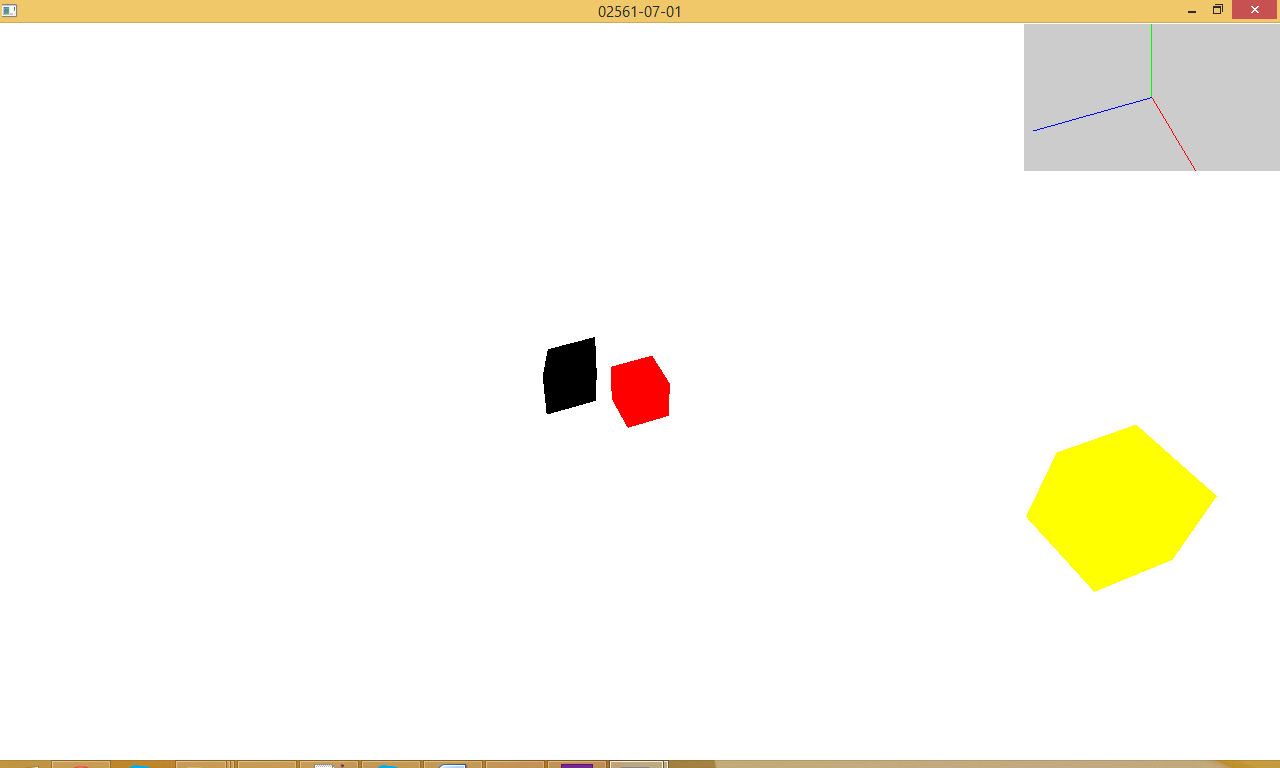
\includegraphics[width=8cm]{../Screenshots/ex-7/1-1.png}
\caption{Point light source shadow}
\label{fig:7-1-1}
\end{figure} 

\subsection{Part b}

You can see my \emph{createShadowProjectionDirectionalLight } implementation below.\\

\begin{lstlisting}
mat4 createShadowProjectionDirectionalLight() {
	mat4 m;
	vec4 newlightPos=10000*lightPos;
                //drag the light source far 
                //far away without changing
                //jts direction.
	m[3][0] = -1.0/(newlightPos[0]-shadowDistance);
	m[3][3] = 0;
 	mat4 shadow=Translate(newlightPos[0],newlightPos[1], 
        newlightPos[2]) * m * Translate(-newlightPos[0],
        -newlightPos[1],-newlightPos[2]);
	return shadow;	
}
\end{lstlisting}

When point source is so far away from the object, the system resembles to a directional light system because the rays coming from far point source become almost parallel. I use this fact to implement directional light source shadows.

The resulting scene can be seen in Figure \ref{fig:7-1-2}.

\begin{figure}[hp]
\centering
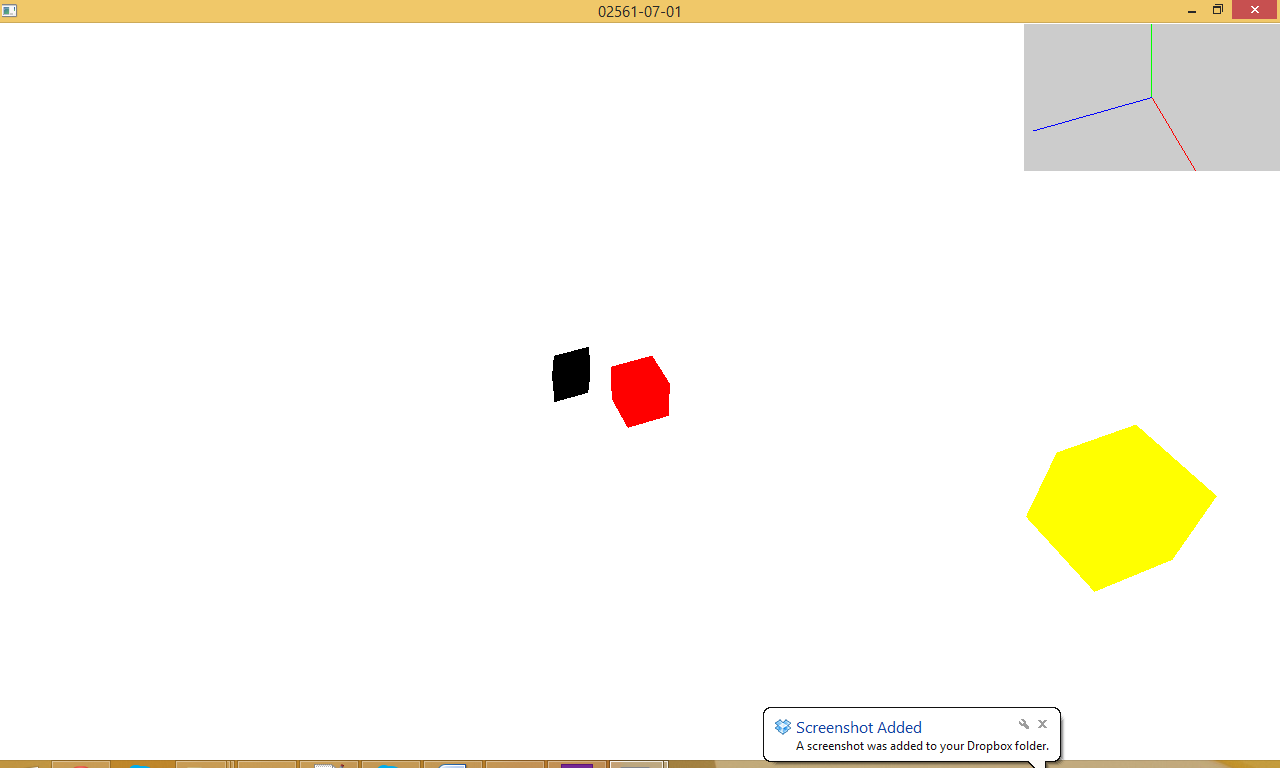
\includegraphics[width=8cm]{../Screenshots/ex-7/1-2.png}
\caption{Directional light source shadow}
\label{fig:7-1-2}
\end{figure} 


\subsection{Part c}
I add the functionality with this simple code fragment:\\
\begin{lstlisting}
	case 'd':
		if(shadowDistance==-4)
			shadowDistance=-8;
		else
			shadowDistance=-4;
		break;
\end{lstlisting}
